\documentclass{report}

\usepackage[a4paper,margin=2cm]{geometry}
\usepackage{fancyhdr}
\usepackage{graphicx}
\usepackage[utf8]{inputenc}
\usepackage[greek,spanish]{babel}
\usepackage{amsmath,amssymb,amsthm,amsfonts}
\usepackage{multicol}
\usepackage{array}
\usepackage{skak}
\usepackage{hyperref}
\usepackage{tikz}
\usepackage{tkz-euclide}
\usepackage{xcolor}
\usepackage{centernot}
\usepackage{float}
\usepackage{scrlayer}
\usepackage{titlesec}
\usepackage{blindtext}
\usepackage{mathrsfs}
\usepackage{color}
\usepackage{pgfplots}
\usetkzobj{all}
\usetikzlibrary{shapes.multipart, positioning, patterns, math}

% Configuración del entorno chapter, section, subsection y subsubsection.
\setcounter{secnumdepth}{3}
\definecolor{gray75}{gray}{0.75}
\newcommand{\hspC}{\hspace{10pt}}
\newcommand{\hspS}{\hspace{5pt}}
\newcommand{\hspSS}{\hspace{2.5pt}}
\newcommand{\hspSSS}{\hspace{1.125pt}}
\titleformat{\chapter}[hang]{\Huge\bfseries}{\textcolor{gray75}{\thechapter}\hspC\textcolor{gray75}{$|$}\hspC}{0pt}{\Huge\bfseries}
\titleformat{\section}[hang]{\Large\bfseries}{\textcolor{gray75}{\thesection}\hspS\textcolor{gray75}{$|$}\hspS}{0pt}{\Large\bfseries}
\titleformat{\subsection}[hang]{\large\bfseries}{\textcolor{gray75}{\thesubsection}\hspSS\textcolor{gray75}{$|$}\hspSS}{0pt}{\large\bfseries}
\titleformat{\subsubsection}[hang]{\normalsize\bfseries}{\textcolor{gray75}{\thesubsubsection}\hspSSS\textcolor{gray75}{$|$}\hspSSS}{0pt}{\normalsize\bfseries}

% Encabezado y pie de página.
\lhead{\textit{Economía}}
\rhead{Nicolás Lemuñir, Daniel Lobos}
\chead{\thepage}
\cfoot{\begin{center}
\includegraphics[width=170mm]{barrauchile.png}\end{center}}
\renewcommand{\headrulewidth}{0.05cm}
\renewcommand{\footrulewidth}{0pt}
\pagestyle{fancy}

% Configuración de párrafos.
\setlength{\parskip}{0.25cm}
\setlength{\parindent}{1cm}

% Comandos simbólicos.
\newcommand{\dom}{\operatorname{dom}}
\newcommand{\rec}{\operatorname{rec}}
\newcommand{\cod}{\operatorname{cod}}
\newcommand{\im}{\operatorname{im}}
\newcommand{\interior}{\operatorname{int}}
\newcommand{\sech}{\operatorname{sech}}
\newcommand{\csch}{\operatorname{csch}}
\newcommand{\id}{\operatorname{id}}
\newcommand{\sgn}{\operatorname{sgn}}
\newcommand{\gr}{\operatorname{gr}}
\renewcommand{\labelenumi}{\textup{(\arabic{enumi})}}
\renewcommand{\labelenumii}{\textup{(\roman{enumii})}}
\renewcommand{\labelitemi}{---}
\renewcommand{\qedsymbol}{$\blacksquare$}
\DeclareSymbolFont{largesymbolsA}{U}{txexa}{m}{n}
\DeclareMathSymbol{\varprod}{\mathop}{largesymbolsA}{16}
\newcommand{\GRAF}{\begin{center}$$\mathfrak{Gr\acute{a}fico}$$\end{center}}

% Comandos para TikZ.
\def\aureo{1.61803}
\tikzstyle{startstop} = [rectangle, rounded corners, minimum width=3cm, minimum height=1cm, text width=6cm, text centered, draw=black]
\tikzstyle{process} = [rectangle, minimum width=3cm, minimum height=1cm, text centered, text width=6 cm, draw=black]
\tikzstyle{arrow} = [thick,->,>=stealth]

% Entornos.
\newcounter{axiom}
\newcounter{theorem}[chapter]
\newcounter{corollary}[theorem]
\newenvironment{axiom}[1]{\refstepcounter{axiom}\noindent\setlength{\parskip}{0pt}\textbf{Axioma~\theaxiom} (#1).\em}{}
\newenvironment{theorem}[1]{\refstepcounter{theorem}\noindent\setlength{\parskip}{0pt}\textbf{Teorema~\thechapter.\thetheorem} (#1).\em}{}
\newenvironment{corollary}{\refstepcounter{corollary}\noindent\setlength{\parskip}{0pt}\textbf{Corolario~\thechapter.\thetheorem.\thecorollary}}{}
\newenvironment{prop}[1]{\refstepcounter{theorem}\noindent\setlength{\parskip}{0pt}\textbf{Proposición~\thechapter.\thetheorem} (#1).}{}
\newenvironment{example}[1]{\noindent\setlength{\parskip}{0pt}\textbf{Ejemplo.} (#1).}{}
\newenvironment{obs}{$\star$ }{}
\newenvironment{definition}[1]{\begin{center}
\begin{tabular}{p{3.5cm} p{12.5cm}}
\textbf{#1} &
}
{\\ \end{tabular}\end{center}}
\newtheorem*{supuesto}{Supuesto}

% Configuración de tablas.
\newcolumntype{C}[1]{%
 >{\vbox to 3ex\bgroup\vfill\centering}%
 m{#1}%
 <{\egroup}} 
\newcolumntype{D}{ >{\centering\arraybackslash} m{30pt} }

% Página en blanco (usar con \newpage\null\thispagestyle{blank}\newpage).
\DeclareNewLayer[foreground,contents={\parbox[b][\layerheight][c]{\layerwidth}{\centering This page was intentionally left blank.}}]{blankpage.fg}
\DeclarePageStyleByLayers{blank}{blankpage.fg}

\begin{document}

\chapter{Introducción: demanda, oferta y equilibrio}

\thispagestyle{fancy}

\section{¿Qué es la economía?}

La economía es el estudio de las elecciones de los agentes y las sociedades en condiciones de escasez. No solo se trata de dinero, sino que también de decidir qué es lo mejor con respecto a los espacios públicos. La economía estudia: qué y cuánto se produce, cómo se produce y cómo se distribuye la producción; pero las respuestas a estas preguntas dependen de la forma en que se organicen las sociedades.

\subsection{Formas de organización}

\begin{enumerate}
\item \textbf{Planificador central:} Un solo agente decide las respuestas a estas tres preguntas. Se debe coordinar a mucha gente, lo que es más complicado en este caso.
\item \textbf{Economía de mercado:} Muchos agentes toman decisiones individuales.
\end{enumerate}

\subsection{El método científico y la economía}

Esencialmente, la economía estudia la forma en que las sociedades deciden qué van a producir, cómo y para quién, con recursos escasos y limitados. Esto se realiza haciendo uso del método científico para generar un modelo o teoría de la realidad. Uno de los principales problemas que enfrenta la economía con respecto al uso del método científico es la dificultad para realizar experimentos, esto, pues el objeto de estudio son personas, o grupos de personas, que tienen voluntad. Por esto, la economía es una ciencia social; sin embargo, queda la posibilidad de los experimentos naturales.

\begin{example}{Valor subjetivo del tiempo}
Un ejemplo de un modelo o teoría microeconómica es el valor subjetivo del tiempo, es decir, que importa en qué se invierte el tiempo de una persona.
\end{example}

\subsubsection{¿De qué depende si una teoría o modelo es valiosa?}

\begin{enumerate}
\item \textbf{Capacidad de predicción:} Lo ideal es que se supongan pocas cosas para entregar un resultado.
\item \textbf{Simplicidad y generalidad:} Debe ser simple para poder ser utilizable y debe ser general, es decir, aplicar a varios casos.
\end{enumerate}

\subsection{Predicción en economía}

\begin{enumerate}
\item \textbf{Microeconomía:} Es el modo en que se toman las decisiones en los hogares y empresas, y cómo ellos interactúan en los diferentes mercados (demanda, oferta, excedentes, elasticidades, eficiencia, costo de oportunidad, etc.)
\item \textbf{Macroeconomía:} Estudia los fenómenos agregados que afectan al conjunto de la economía (crecimiento, ciclo, inflación, desempleo, ahorro, inversión, cuenta corriente, exportaciones, importaciones, saldo fiscal, dinero, etc.)
\end{enumerate}

\subsection{Simplicidad de los modelos y rol de los supuestos}

Los supuestos juegan un rol fundamental en la formulación de teorías y modelos:
\setlength{\parskip}{0cm}
\begin{enumerate}
\item permiten simplificar el problema;
\item pueden capturar parcialmente la realidad;
\item para predecir relativamente bien, muchas veces basta con capturar los elementos esenciales del problema, obviando otros.
\end{enumerate}
\setlength{\parskip}{0.25cm}

Además, es importante conocer bien los supuestos detrás de cada modelo, especialmente en economía. Muchas veces algunos supuestos pueden parecer poco realistas, pero aun así permitir una buena predicción.

\subsection{Flujo circular de la economía}

\begin{enumerate}
\item Las familias compran y consumen bienes y servicios.
\item El mercado de bienes y servicios recibe y entrega ingresos a empresas.
\item Las empresas entregan salarios a familias.
\end{enumerate}

\begin{figure}[H]
\begin{center}
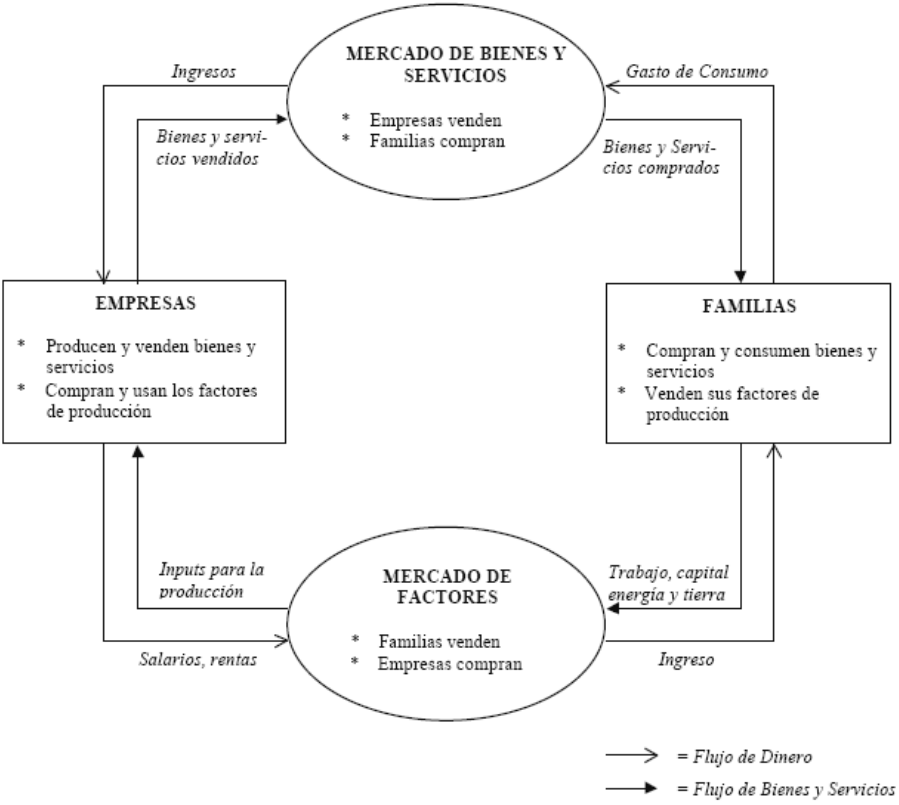
\includegraphics[width=12cm]{flujocircular.png}
\end{center}
\caption{Flujo circular}
\end{figure}

\subsection{Análisis positivo y análisis normativo}

\begin{enumerate}
\item \textbf{Economía positiva}
\begin{enumerate}
\item Se analizan los hechos y se entregan resultados objetivos.
\item Descripción de causas y efectos.
\item No hay un juicio de valor sino un afán de entender y predecir.
\item Se puede verificar con información real.
\end{enumerate}
\item \textbf{Economía normativa}
\begin{enumerate}
\item Es como debiese ser la economía.
\item Hay juicios de valor basados en consideraciones políticas, religiosas, etc.
\end{enumerate}
\end{enumerate}

\subsection{\textit{Trade-offs}}

Los agentes enfrentan \textit{trade-offs}. El enfoque económico consiste en comparar costos con beneficios para tratar de entender las decisiones; pero ¿cómo se miden los costos y beneficios?
\begin{enumerate}
\item \textbf{Costos directos:} El valor en-sí.
\item \textbf{Costos de oportunidad:} El valor de la mejor alternativa que se descarta al tomar una decisión.
\end{enumerate}

\subsection{Frontera de posibilidades de producción (FPP)}

Un modelo que captura que los recursos son escasos y por ende debiese mostrar los costos de oportunidad es la FPP. Es una forma que muestra en un gráfico la combinación de bienes y servicios que se producen si la cantidad de recursos se usa eficientemente.\\

\begin{example}{Ejemplo de Eisenhower}
Se supone que una cierta cantidad de mano de obra puede usarse para producir armamento.
\begin{center}
\begin{tikzpicture}
\draw [latex-latex] (-1, 0) -- (3, 0);
\draw [latex-latex] (0, -1) -- (0, 3);
\draw [domain=0:2, smooth, color=red] plot (\x,{sqrt(4-\x*\x)});
\filldraw (0.5, 0.5) circle (1pt) node[above] {$A$};
\filldraw (1, {sqrt(3)}) circle (1pt) node[above] {$B$};
\filldraw ({sqrt(3)}, 1) circle (1pt) node[above] {$C$};
\filldraw (2.5, 2.5) circle (1pt) node[above] {$D$};
\filldraw (3, 0) circle (0pt) node[below] {$v\ \text{(viviendas)}$};
\filldraw (0, 3) circle (0pt) node[left] {$a\ \text{(armas)}$};
\end{tikzpicture}
\end{center}
\end{example}

La posición $A$ es factible, pero no eficiente; la posición $B$ y $C$ son eficientes; y la posición $D$ es infactible, pues usa más recursos de los disponibles. El costo de oportunidad de subir desde $a_C$ hasta $a_B$ es $v_C$ a $v_B$. La derivada de la FPP es el costo de oportunidad: al variar $A$, el costo de oportunidad es $0$, mientras que al cambiar $D$, el costo de oportunidad no existe.

\subsection{La mano invisible}

\begin{definition}{Insumos}
Capital y trabajo (máquinas y personas).
\end{definition}

\begin{center}
<<\textit{Generalmente, un individuo no trata de promover el bien público, lo único que busca es su propio bienestar. Al hacerlo, una mano invisible lo lleva a promover un fin que no estaba en sus intenciones; al buscar su propio bienestar, a menudo un individuo promueve el de la sociedad más eficientemente que si realmente intentara hacerlo}>>.
\end{center}
\begin{flushright}
Adam Smith. 1776. \textit{La riqueza de las naciones}.
\end{flushright}

Es decir, una economía de mercado en que miles de agentes toman decisiones individuales buscando su propio bienestar, llevaría a la sociedad a la FPP. Esto queda por demostrar.

\begin{enumerate}
\item \textbf{Análisis marginal:} Muchas veces las decisiones de los agentes involucran pequeños cambios sobre planes de acción ya existentes. Hay costos que en algunos casos no deben ser tomados en cuenta: no son relevantes al momento de la decisión.
\item \textbf{Costos hundidos:} Son los costos no recuperables al momento de tomar una decisión. Estos no afectan la decisión de cuánto producir, pero sí afectan la decisión de si producir o no.
\end{enumerate}

\section{Sistema de mercado}

\subsection{Ingredientes de un sistema de mercado}

\begin{enumerate}
\item \textbf{Consumidores:} Tienen preferencias racionales y consistentes respecto a canastas de bienes, y compran bienes basados en estas preferencias sujetos a su restricción presupuestaria.
\item \textbf{Productores:} Poseen la tecnología para transformar insumos (materias primas, factores) en bienes que son deseables por los consumidores.
\item \textbf{Mercado:} Los productores y consumidores se encuentran en un mercado para intercambiar bienes por dinero.
\end{enumerate}

\subsection{¿Qué es un mercado?}

Un mercado es cualquier proceso mediante el cual consumidores y productores intercambian bienes. El dinero de los consumidores para poder comprar sale del flujo circular de la economía.

\subsection{Modelo competencia perfecta}

\begin{enumerate}
\item \textbf{Muchos consumidores:} Toman el precio como dato y compran según preferencia y presupuesto.
\item \textbf{Muchos productores:} Toman el precio como dato (insumo y bienes) y maximizan ganancias.
\item \textbf{Muchos productores de insumo:} No afectan el precio de los factores (materias primas e insumos).
\end{enumerate}

En conclusión, los agentes creen que no pueden afectar los precios, pero sí pueden hacerlo.

\subsubsection{Casos extremos (no se cumple el supuesto)}

\begin{enumerate}
\item \textbf{Monopolio:} Es un solo mercado productor.
\item \textbf{Monopsonio:} Es un solo mercado consumidor (usualmente se da en el mercado del trabajo).
\end{enumerate}

\begin{center}
\begin{tikzpicture}
\draw [|-|] (-6, 0) -- (6, 0);
\filldraw (0, -3pt) -- (0, 3pt) node [below, yshift=-3pt] {Oligopolios (duopolio) (2)};
\foreach \x in {-6} \draw [shift={(\x,0)}, color=black] (0, 0) -- (0, 0) node [below] {Competencia perfecta (1)};
\foreach \x in {6} \draw [shift={(\x,0)}, color=black] (0, 0) -- (0, 0) node [below] {Monopolios};
\end{tikzpicture}
\end{center}

\begin{enumerate}
\item Muchos productores.
\item Los productos afectan relativamente los precios (aerolíneas, farmacias, etc). Hay pocos productores.
\end{enumerate}

\begin{obs}
Los oligopsonios son similares a los monopsonios.
\end{obs}

\subsection{Bienes}

\begin{definition}{Bienes homogéneos}
Son bienes que se parecen, pero son diferentes, están en un mismo grupo. Se puede sustituir uno con el otro.
\end{definition}

\subsection{Equilibrio competitivo}

Es el vector de precios (uno para cada bien) tal que la cantidad ofertada y la cantidad demandada es la misma. Se relaciona con el ajuste de precio.

\begin{example}{Equilibrio competitivo y el pan}
Los panes de todos los productores responden a un único precio, por lo que son bienes homogéneos. Tanto productores como consumidores responden al precio (si se agrupan).
\end{example}

\subsection{La función (o curva) de oferta}

Es el número de unidades de un bien que, para un precio dado, los productores desean vender $Q_S\!\left(P,\mathbf{x}\right)$ o $Q_O\!\left(P,\mathbf{x}\right)$, donde $\mathbf{x}$ son otras variables distintas al precio.

\begin{center}
\begin{tikzpicture}
\draw [latex-latex] (-1, 0) -- (3, 0);
\draw [latex-latex] (0, -1) -- (0, 3);
\draw [domain=0:2.5, smooth, color=red] plot (\x,{1/3*\x^2});
\foreach \x in {1} \draw  [shift={(\x, 0)}, color=black] (0, -3pt) -- (0, 3pt) node [below, yshift=-3pt] {20};
\foreach \x in {2} \draw  [shift={(\x, 0)}, color=black] (0, -3pt) -- (0, 3pt) node [below, yshift=-3pt] {40};
\foreach \x in {1/3} \draw  [shift={(0, \x)}, color=black] (-3pt, 0) -- (3pt, 0) node [left, xshift=-3pt] {200};
\foreach \x in {4/3} \draw  [shift={(0, \x)}, color=black] (-3pt, 0) -- (3pt, 0) node [left, xshift=-3pt] {300};
\draw [dashed] (1, 0) -- (1, 1/3);
\draw [dashed] (2, 0) -- (2, 4/3);
\draw [dashed] (0, 1/3) -- (1, 1/3);
\draw [dashed] (0, 4/3) -- (2, 4/3);
\filldraw (3, 0) circle (0pt) node[below, xshift=2cm] {$Q\ \text{(cant. de prod. vendidos)}$};
\filldraw (0, 3) circle (0pt) node[left] {$P\ \text{(precio)}$};
\end{tikzpicture}
\end{center}

En general, cuando hay $n$ empresas, la oferta agregada (oferta total del mercado) es
$$Q_S\!\left(P,\mathbf{x}\right)=\sum_{i=1}^n q_{Si}\!\left(P,\mathbf{x}\right)\text{;}$$
con $q_{Si}$ la oferta individual de la empresa $i$-ésima.

\subsection{La función (o curva) de demanda}

Indica, para cada precio, la cantidad que los consumidores comprarán $Q_D\!\left(P,\mathbf{x}\right)$, donde $\mathbf{x}$ son otras variables distintas de precio.

\begin{center}
\begin{tikzpicture}
\draw [latex-latex] (-1, 0) -- (3, 0);
\draw [latex-latex] (0, -1) -- (0, 3);
\draw [domain=0.4:2.5, smooth, color=red] plot (\x,{1/\x});
\foreach \x in {0.75} \draw  [shift={(\x, 0)}, color=black] (0, -3pt) -- (0, 3pt) node [below, yshift=-3pt] {10};
\foreach \x in {2.25} \draw  [shift={(\x, 0)}, color=black] (0, -3pt) -- (0, 3pt) node [below, yshift=-3pt] {20};
\foreach \x in {1.33} \draw  [shift={(0, \x)}, color=black] (-3pt, 0) -- (3pt, 0) node [left, xshift=-3pt] {300};
\foreach \x in {0.44} \draw  [shift={(0, \x)}, color=black] (-3pt, 0) -- (3pt, 0) node [left, xshift=-3pt] {200};
\draw [dashed] (0.75, 0) -- (0.75, 1.33);
\draw [dashed] (2.25, 0) -- (2.25, 0.44);
\draw [dashed] (0, 1.33) -- (0.75, 1.33);
\draw [dashed] (0, 0.44) -- (2.25, 0.44);
\filldraw (3, 0) circle (0pt) node[below, xshift=2cm] {$Q\ \text{(cant. de prod. vendidos)}$};
\filldraw (0, 3) circle (0pt) node[left] {$P\ \text{(precio)}$};
\end{tikzpicture}
\end{center}

\begin{obs}
\textbf{Bien Giffen:} A más precio, más demanda.
\end{obs}

En general, cuando hay $n$ consumidores, la demanda agregada es
$$Q_D\!\left(P,\mathbf{x}\right)=\sum_{i=1}^nq_{Di}\!\left(P,\mathbf{x}\right)\text{;}$$
con $q_{Di}$ la demanda individual del consumidor $i$-ésimo.

\subsubsection{¿Qué sucede con la curva de demanda si aumentan los ingresos?}

La curva de demanda se expande si sube el ingreso para bienes normales (por ejemplo, lomo vetado), es decir, aumenta la demanda, mientras que se contrae para bienes inferiores (por ejemplo, jugo en polvo), es decir, disminuye la demanda.

\begin{multicols}{2}
\begin{figure}[H]
\begin{center}
\begin{tikzpicture}
\draw [latex-latex] (-1, 0) -- (3, 0);
\draw [latex-latex] (0, -1) -- (0, 3);
\draw [-latex, thick] (0.76, 1.33) -- (1.5, 1.33);
\draw [domain=0.8:2.5, smooth, color=red] plot (\x,{2*1/\x});
\draw [domain=0.4:2.1, smooth, color=blue] plot (\x,{2*1/(\x+0.4)-0.4});
\foreach \x in {0.76} \draw  [shift={(\x, 0)}, color=black] (0, -3pt) -- (0, 3pt) node [below, yshift=-3pt] {$Q_i$};
\foreach \x in {1.5} \draw  [shift={(\x, 0)}, color=black] (0, -3pt) -- (0, 3pt) node [below, yshift=-3pt] {$Q_f$};
\foreach \x in {1.33} \draw  [shift={(0, \x)}, color=black] (-3pt, 0) -- (3pt, 0) node [left, xshift=-3pt] {$P^*$};
\draw [dashed] (1.5, 0) -- (1.5, 1.33);
\draw [dashed] (0.76, 0) -- (0.76, 1.33);
\draw [dashed] (0, 1.33) -- (0.76, 1.33);
\filldraw (3, 0) circle (0pt) node[below] {$Q$};
\filldraw (0, 3) circle (0pt) node[left] {$P$};
\end{tikzpicture}
\end{center}
\caption{Bienes normales}
\end{figure}
\begin{figure}[H]
\begin{center}
\begin{tikzpicture}
\draw [latex-latex] (-1, 0) -- (3, 0);
\draw [latex-latex] (0, -1) -- (0, 3);
\draw [latex-, thick] (0.76, 1.33) -- (1.5, 1.33);
\draw [domain=0.8:2.5, smooth, color=blue] plot (\x,{2*1/\x});
\draw [domain=0.4:2.1, smooth, color=red] plot (\x,{2*1/(\x+0.4)-0.4});
\foreach \x in {0.76} \draw  [shift={(\x, 0)}, color=black] (0, -3pt) -- (0, 3pt) node [below, yshift=-3pt] {$Q_f$};
\foreach \x in {1.5} \draw  [shift={(\x, 0)}, color=black] (0, -3pt) -- (0, 3pt) node [below, yshift=-3pt] {$Q_i$};
\foreach \x in {1.33} \draw  [shift={(0, \x)}, color=black] (-3pt, 0) -- (3pt, 0) node [left, xshift=-3pt] {$P^*$};
\draw [dashed] (1.5, 0) -- (1.5, 1.33);
\draw [dashed] (0.76, 0) -- (0.76, 1.33);
\draw [dashed] (0, 1.33) -- (0.76, 1.33);
\filldraw (3, 0) circle (0pt) node[below] {$Q$};
\filldraw (0, 3) circle (0pt) node[left] {$P$};
\end{tikzpicture}
\end{center}
\caption{Bienes inferiores}
\end{figure}
\end{multicols}

\subsubsection{¿Qué sucede con la curva de demanda si cambia el precio de otro bien?}

\begin{enumerate}
\item Si el bien es \textit{sustituto}, entonces el precio aumenta y $Q_D$ se expande (por ejemplo, el té y el café).
\item Si el bien es \textit{complementario}, entonces el precio aumenta y $Q_D$ se contrae (por ejemplo, el pan y la mantequilla).
\end{enumerate}

\subsection{Equilibrio de mercado (competitivo)}

\begin{obs}
En este gráfico, el par $\left(Q^*,P^*\right)$ es el equilibrio de mercado (oferta y demanda agregada).
\end{obs}

\begin{center}
\begin{tikzpicture}
\draw [latex-latex] (-1, 0) -- (3, 0);
\draw [latex-latex] (0, -1) -- (0, 3);
\draw [domain=0.5:2.5, smooth, color=red] plot (\x,\x);
\draw [domain=0.5:2.5, smooth, color=red] plot (\x,-\x+3);
\foreach \x in {1.5} \draw  [shift={(\x, 0)}, color=black] (0, -3pt) -- (0, 3pt) node [below, yshift=-3pt] {$Q^*$};
\foreach \x in {1.5} \draw  [shift={(0, \x)}, color=black] (-3pt, 0) -- (3pt, 0) node [left, xshift=-3pt] {$P^*$};
\draw [dashed] (1.5, 0) -- (1.5, 1.5);
\draw [dashed] (0, 1.5) -- (1.5, 1.5);
\filldraw (3, 0) circle (0pt) node[below, xshift=2cm] {$Q\ \text{(cant. de prod. vendidos)}$};
\filldraw (0, 3) circle (0pt) node[left] {$P\ \text{(precio)}$};
\end{tikzpicture}
\end{center}

\begin{obs}
Este gráfico es el caso exceso de oferta $\overline{Q}_S-\overline{Q}_D>0$.
\end{obs}

\begin{center}
\begin{tikzpicture}
\draw [latex-latex] (-1, 0) -- (3, 0);
\draw [latex-latex] (0, -1) -- (0, 3);
\draw [domain=0.5:2.5, smooth, color=red] plot (\x,\x);
\draw [domain=0.5:2.5, smooth, color=red] plot (\x,-\x+3);
\foreach \x in {1} \draw  [shift={(\x, 0)}, color=black] (0, -3pt) -- (0, 3pt) node [below, yshift=-3pt] {$\overline{Q}_D$};
\foreach \x in {2} \draw  [shift={(\x, 0)}, color=black] (0, -3pt) -- (0, 3pt) node [below, yshift=-3pt] {$\overline{Q}_S$};
\foreach \x in {2} \draw  [shift={(0, \x)}, color=black] (-3pt, 0) -- (3pt, 0) node [left, xshift=-3pt] {$\overline{P}$};
\draw [dashed] (0, 2) -- (2, 2);
\draw [dashed] (1, 0) -- (1, 2);
\draw [dashed] (2, 0) -- (2, 2);
\filldraw (3, 0) circle (0pt) node[below, xshift=2cm] {$Q\ \text{(cant. de prod. vendidos)}$};
\filldraw (0, 3) circle (0pt) node[left] {$P\ \text{(precio)}$};
\end{tikzpicture}
\end{center}

\begin{obs}
Este gráfico es el caso exceso de demanda $\underline{Q}_D-\underline{Q}_S>0$.
\end{obs}

\begin{center}
\begin{tikzpicture}
\draw [latex-latex] (-1, 0) -- (3, 0);
\draw [latex-latex] (0, -1) -- (0, 3);
\draw [domain=0.5:2.5, smooth, color=red] plot (\x,\x);
\draw [domain=0.5:2.5, smooth, color=red] plot (\x,-\x+3);
\foreach \x in {1} \draw  [shift={(\x, 0)}, color=black] (0, -3pt) -- (0, 3pt) node [below, yshift=-3pt] {$\underline{Q}_S$};
\foreach \x in {2} \draw  [shift={(\x, 0)}, color=black] (0, -3pt) -- (0, 3pt) node [below, yshift=-3pt] {$\underline{Q}_D$};
\foreach \x in {1} \draw  [shift={(0, \x)}, color=black] (-3pt, 0) -- (3pt, 0) node [left, xshift=-3pt] {$\underline{P}$};
\draw [dashed] (0, 1) -- (2, 1);
\draw [dashed] (1, 0) -- (1, 1);
\draw [dashed] (2, 0) -- (2, 1);
\filldraw (3, 0) circle (0pt) node[below, xshift=2cm] {$Q\ \text{(cant. de prod. vendidos)}$};
\filldraw (0, 3) circle (0pt) node[left] {$P\ \text{(precio)}$};
\end{tikzpicture}
\end{center}

\subsection{Análisis \textit{cæterīs pāribus}}

Corresponde a analizar el efecto de una variable asumiendo todas las demás constantes. La idea del análisis \textit{cæterīs pāribus} es identificar efectos haciendo uso de herramientas como las derivadas parciales.

\begin{enumerate}
\item \textbf{Aumento de ingreso:}
\begin{enumerate}
\item $\uparrow$ demanda para bienes normales.
\item $\downarrow$ demanda para bienes inferiores.
\end{enumerate}
\item \textbf{Aumento precio de otro bien:}
\begin{enumerate}
\item $\uparrow$ demanda para bienes sustitutos
\item $\downarrow$ demanda para bienes complementarios.
\end{enumerate}
\end{enumerate}

Haciendo el análisis \textit{cæterīs pāribus} se puede saber qué pasa con las curvas de oferta y demanda, y además qué pasa con respecto al precio y cantidad de equilibrio.

\subsubsection{¿Qué cosas afectan a la curva de oferta aparte del precio del bien?}

\begin{enumerate}
\item \textbf{Precio del insumo:} Si suben, la curva se contrae.
\item \textbf{Cantidad de productos:} Que dependerá de la tecnología o el clima.
\end{enumerate}

\subsection{Estática comparativa}

\begin{example}{Mercado de las verduras}
Si una ola de frío destruye la producción de lechugas de varios productores, entonces el precio aumenta y la oferta disminuye.
\begin{center}
\begin{tikzpicture}
\draw [latex-latex] (-1, 0) -- (3, 0);
\draw [latex-latex] (0, -1) -- (0, 3);
\draw [domain=0.8:2.5, smooth, color=red] plot (\x,{-2/(\x-3-0.4)+0.4});
\draw [domain=1.2:2.9, smooth, color=blue] plot (\x,{-2/(\x-3-0.8)});
\draw [domain=0.8:2.9, smooth, color=red] plot (\x,{2*1/(\x+0.3)+0.4});
\draw [latex-, thick] (1.55, 1.48) -- (2.15, 1.22);
\foreach \x in {1.55} \draw  [shift={(\x, 0)}, color=black] (0, -3pt) -- (0, 3pt) node [below, yshift=-3pt] {$Q_f$};
\foreach \x in {2.15} \draw  [shift={(\x, 0)}, color=black] (0, -3pt) -- (0, 3pt) node [below, yshift=-3pt] {$Q_i$};
\foreach \x in {1.22} \draw  [shift={(0, \x)}, color=black] (-3pt, 0) -- (3pt, 0) node [left, xshift=-3pt, yshift=-3pt] {$P_i$};
\foreach \x in {1.48} \draw  [shift={(0, \x)}, color=black] (-3pt, 0) -- (3pt, 0) node [left, xshift=-3pt, yshift=3pt] {$P_f$};
\draw [dashed] (2.15, 0) -- (2.15, 1.22);
\draw [dashed] (1.55, 0) -- (1.55, 1.48);
\draw [dashed] (0, 1.22) -- (2.15, 1.22);
\draw [dashed] (0, 1.48) -- (1.55, 1.48);
\filldraw (3, 0) circle (0pt) node[below, xshift=17pt] {$Q\ \text{(lechugas)}$};
\filldraw (0, 3) circle (0pt) node[left] {$P$};
\end{tikzpicture}
\end{center}
\end{example}

\begin{example}{Estufas e invierno}
Se aprovecha la ola de frío, con lo que el precio de las estufas aumenta y la oferta también.
\begin{center}
\begin{tikzpicture}
\draw [latex-latex] (-1, 0) -- (3, 0);
\draw [latex-latex] (0, -1) -- (0, 3);
\draw [domain=1:2.5, smooth, color=red] plot (\x,{-2/(-\x-3.8+4)});
\draw [domain=0.6:2.1, smooth, color=blue] plot (\x,{-2/(-\x-3.8+3.6)-0.4});
\draw [domain=0.6:2.9, smooth, color=red] plot (\x,{2*1/(-\x+0.3+4)+0.4});
\draw [-latex, thick] (1.19, 1.04) -- (1.84, 1.21);
\foreach \x in {1.19} \draw  [shift={(\x, 0)}, color=black] (0, -3pt) -- (0, 3pt) node [below, yshift=-3pt] {$Q_i$};
\foreach \x in {1.84} \draw  [shift={(\x, 0)}, color=black] (0, -3pt) -- (0, 3pt) node [below, yshift=-3pt] {$Q_f$};
\foreach \x in {1.04} \draw  [shift={(0, \x)}, color=black] (-3pt, 0) -- (3pt, 0) node [left, xshift=-3pt, yshift=-3pt] {$P_i$};
\foreach \x in {1.21} \draw  [shift={(0, \x)}, color=black] (-3pt, 0) -- (3pt, 0) node [left, xshift=-3pt, yshift=3pt] {$P_f$};
\draw [dashed] (1.84, 0) -- (1.84, 1.21);
\draw [dashed] (1.19, 0) -- (1.19, 1.04);
\draw [dashed] (0, 1.21) -- (1.84, 1.21);
\draw [dashed] (0, 1.04) -- (1.19, 1.04);
\filldraw (3, 0) circle (0pt) node[below, xshift=17pt] {$Q\ \text{(estufas)}$};
\filldraw (0, 3) circle (0pt) node[left] {$P$};
\end{tikzpicture}
\end{center}
\end{example}

En el primer ejemplo existe un desplazamiento de la curva de oferta sobre la curva de demanda, mientras que en el segundo ejemplo existe un desplazamiento de la curva de demanda sobre la curva de oferta.\\

\begin{example}{Arriendos en el litoral central}
En verano, suben los precios hasta llegar a una restricción, de capacidad, es decir, hay demasiada demanda que la oferta no puede cumplir.
\begin{center}
\begin{tikzpicture}
\draw [latex-latex] (-1, 0) -- (3, 0);
\draw [latex-latex] (0, -1) -- (0, 3);
\draw [domain=0.4:2.35, smooth, color=red] plot (\x,{1/(-\x+2.7)});
\draw [dashed] (2.6, -1) -- (2.6, 3);
\filldraw (3, 0) circle (0pt) node[below, xshift=19pt] {$Q\ \text{(arriendos)}$};
\filldraw (0, 3) circle (0pt) node[left] {$P$};
\end{tikzpicture}
\end{center}
\end{example}

\subsection{Rol de los precios}

\begin{enumerate}
\item Información que asegura consistencia de decisión de firmas y consumidores.
\item Señalan qué es relativamente escaso o abundante.
\item Permiten racionar bienes escasos (debe ser racionado entre potenciales consumidores; los que están dispuestos a pagar obtienen el bien).
\end{enumerate}

\section{Elasticidades}

No solo interesa la dirección de los cambios sino que también la magnitud de estos.

\begin{center}
\begin{tikzpicture}
\draw [latex-latex] (-1, 0) -- (3, 0);
\draw [latex-latex] (0, -1) -- (0, 3);
\draw [domain=0.5:2.5, smooth, color=red] plot (\x,{0.75*\x+0.5}) node [above right] {$Q_S^0$};
\draw [domain=0.8:2.8, smooth, color=red] plot (\x,{0.75*(\x-0.3)-0.3}) node [above right] {$Q_S^1$};
\draw [domain=0.6:2.7, smooth, color=red] plot (\x,{-0.5*\x+2});
\draw [domain=0.6:2.5, smooth, color=red, thick] plot (\x,{-1.7561*(\x-1.2)+1.4});
\draw [dashed] (1.2, 0) -- (1.2, 1.4);
\draw [dashed] (0, 1.4) -- (1.2, 1.4);
\draw [dashed] (2.02, 0) -- (2.02, 0.99);
\draw [dashed] (0, 0.99) -- (2.02, 0.99);
\draw [dashed, thick] (1.61, 0) -- (1.61, 0.68);
\draw [dashed, thick] (0, 0.68) -- (1.61, 0.68);
\filldraw (1.2, 1.4) circle (1pt) node[above] {$E^0$};
\filldraw (1.61, 0.68) circle (1pt) node[right] {$E^1$};
\foreach \x in {1.2} \draw  [shift={(\x, 0)}, color=black] (0, -3pt) -- (0, 3pt) node [below, yshift=-3pt, xshift=-3pt] {$Q_0$};
\foreach \x in {1.61} \draw  [shift={(\x, 0)}, color=black] (0, -3pt) -- (0, 3pt) node [below, yshift=-3pt] {$\bar{Q}_1$};
\foreach \x in {2.02} \draw  [shift={(\x, 0)}, color=black] (0, -3pt) -- (0, 3pt) node [below, yshift=-3pt, xshift=3pt] {$Q_1$};
\foreach \x in {1.4} \draw  [shift={(0, \x)}, color=black] (-3pt, 0) -- (3pt, 0) node [left, xshift=-3pt, yshift=3pt] {$P_0$};
\foreach \x in {0.99} \draw  [shift={(0, \x)}, color=black] (-3pt, 0) -- (3pt, 0) node [left, xshift=-3pt, yshift=3pt] {$P_1$};
\foreach \x in {0.68} \draw  [shift={(0, \x)}, color=black] (-3pt, 0) -- (3pt, 0) node [left, xshift=-3pt] {$\bar{P}_1$};
\filldraw (3, 0) circle (0pt) node[below, xshift=17pt] {$Q$};
\filldraw (0, 3) circle (0pt) node[left] {$P$};
\end{tikzpicture}
\end{center}

La magnitud de los cambios depende de las pendientes de las curvas de oferta y demanda, en efecto,
$$\frac{\Delta Q_D}{\Delta P}=\frac{Q_D^1-Q_D^0}{P^1-P^0}=\frac{Q_D\!\left(P^1\right)-Q_D\!\left(P^0\right)}{P^1-P^0}\text{.}$$

Existe un problema con la medida en unidades de $Q$, es difícil comparar entre bienes. No se pueden comparar precios con manzanas, entonces, ¿cómo tener una medida sin unidades? Se medirá en porcentaje.

$$\frac{\dfrac{\Delta Q_D}{Q_D^0}}{\dfrac{\Delta P}{P^0}}=\frac{\dfrac{Q_D^1-Q_D^0}{Q_D^0}}{\dfrac{P^1-P^0}{P^0}}=\frac{Q_D\!\left(P^1\right)-Q_D\!\left(P^0\right)}{P^1-P^0}\frac{P^0}{Q_D\!\left(P^0\right)}\text{.}$$

\begin{definition}{Elasticidad-precio}
La elasticidad-precio, o elasticidad de la demanda con respecto al precio, está dada por la fórmula
$$E_{Q_D,P}\!\left(P\right)=\frac{\partial Q_D\!\left(P\right)}{\partial P}\frac{P}{Q_D\!\left(P\right)}\text{,}$$
lo que significa que la elasticidad-precio de la demanda porcentual es la cantidad demandada cuando el precio varía un 1\%.
\end{definition}

\begin{obs}
El signo de $E_{Q_D,P}$ es negativo.
\end{obs}

\begin{obs}
El valor de $E_{Q_D,P}$ depende del precio al que se evalúa, es decir, es una función de $P$.
\end{obs}

\begin{definition}{Demanda elástica}
Se dice que la demanda por un bien con respecto a su precio es elástica si y solo si $E_{Q_D,P}<-1$, es decir, la demanda se contrae. En este caso, la demanda es sensible al precio, y un aumento del 1\% del precio genera una disminución de más de un 1\% de la demanda.
\end{definition}

\begin{definition}{Demanda inelástica}
Se dice que la demanda por un bien con respecto a su precio es inelástica si y solo si $E_{Q_D,P}>-1$. En este caso, la demanda es insensible al precio, y un aumento del 1\% del precio genera una disminución de menos de un 1\% de la demanda.
\end{definition}

\begin{definition}{Demanda unitaria}
Se dice que la demanda por un bien con respecto a su precio es unitaria si y solo si $E_{Q_D,P}=-1$.
\end{definition}

\subsection{Casos extremos de elasticidad}

\begin{enumerate}
\item Curva de demanda perfectamente inelástica ($E_{Q_D,P}=0$):
\begin{center}
\begin{tikzpicture}
\draw [latex-latex] (-1, 0) -- (3, 0);
\draw [latex-latex] (0, -1) -- (0, 3);
\draw [domain=0:2.9, smooth, color=red] plot (1,\x) node [above right] {$Q_D\!\left(P\right)$};
\filldraw (3, 0) circle (0pt) node[below] {$Q$};
\filldraw (0, 3) circle (0pt) node[left] {$P$};
\end{tikzpicture}
\end{center}
\item Curva de demanda perfectamente elástica ($E_{Q_D,P}\to\infty$):
\begin{center}
\begin{tikzpicture}
\draw [latex-latex] (-1, 0) -- (3, 0);
\draw [latex-latex] (0, -1) -- (0, 3);
\draw [domain=0:2.9, smooth, color=red] plot (\x,1) node [above right] {$Q_D\!\left(P\right)$};
\filldraw (3, 0) circle (0pt) node[below] {$Q$};
\filldraw (0, 3) circle (0pt) node[left] {$P$};
\end{tikzpicture}
\end{center}
\end{enumerate}

\subsection{¿Cómo varían los ingresos?}

Los ingresos son $PQ_D\!\left(P\right)$. Para saber cómo varían se debe derivar esta función con respecto al precio:
\begin{alignat*}{2}
\frac{\partial\left(PQ_D\!\left(P\right)\right)}{\partial P}&=Q_D\!\left(P\right)+\frac{\partial Q_D\!\left(P\right)}{\partial P}P \\
&=Q_D\!\left(P\right)\left(1+\frac{\partial Q_D\!\left(P\right)}{\partial P}\frac{P}{Q_D\!\left(P\right)}\right)\\
&=Q_D\!\left(P\right)\left(1+E_{Q_D,P}\right)\text{.}
\end{alignat*}

Los ingresos por venta aumentan (derivada positiva) cuando aumenta el precio si y solo si $E_{Q_D,P}>-1$, es decir, si la demanda es inelástica.

\subsection{Determinantes de la elasticidad del precio de la demanda}

\begin{enumerate}
\item \textbf{Posibilidades de sustitución:}
\begin{enumerate}
\item Si hay sust. cercanos.
\item Si aumenta el precio de $x$, entonces los consumidores cambian de bien.
\item Se espera que $x$ sea elástica.
\end{enumerate}
\item \textbf{Horizonte de análisis:} Es cuánto tiempo demora el equilibrio en emerger.
\end{enumerate}

\subsection{Elasticidad-ingreso de la demanda}

$$E_{Q_D,I}=\frac{\partial Q_D}{\partial I}\frac{I}{Q_D}\text{,}$$
relaciona cuánto varía la cantidad demandada si el ingreso aumenta un 1\%.

\begin{definition}{Tipos de bienes}
$$\begin{matrix}
E_{Q_D,I}>0 & \text{Bienes normales.} \\
E_{Q_D,I}<0 & \text{Bienes inferiores.} \\
E_{Q_D,I}>1 & \text{Bienes de lujo.} \\
E_{Q_D,I}<1 & \text{Bienes de primera necesidad.}
\end{matrix}$$
\end{definition}

\begin{obs}
Con respecto a los bienes de primera necesidad; a pesar de que aumenta el ingreso, no se necesita una mayor cantidad.
\end{obs}

\chapter{Demanda}

\thispagestyle{fancy}

\GRAF

\section{Teoría de la preferencia de los consumidores}

Se busca modelar o entender cómo un individuo con ingreso $I$ selecciona qué comprar.

\begin{enumerate}
    \item Simplificación para exposición: 2 bienes, $X$ e $Y$.
    \item $x$ cantidad del bien $X$.
    \item $y$ cantidad del bien $Y$.
    \item $v = \left(x, y\right)$ canasta de bienes.
\end{enumerate}

\begin{obs}
    No se quiere decir que $v_1=\left(x_1,y_1\right)$ o $v_2=\left(x_2, y_2\right)$ hace feliz a un individuo. Solo se quiere saber cuál canasta prefiere.
\end{obs}

\subsection {Relación $\mathcal{P}$}

Se define la relación $\mathcal{P}$ como sigue

$$v_1=\left(x_1, y_1\right)\ \mathcal{P}\ v_2=\left(x_2, y_2\right) \Leftrightarrow\text{ el consumidor prefiere la canasta $v_1$ a la canasta $v_2$.}$$

\begin{obs} 
    A veces se usa $\succ$ en vez de $\mathcal{P}$, es decir, $v_1\succ v_2$.
\end{obs}

\begin{obs} 
    Cuando existe una indiferencia sobre qué canasta se prefiere se utiliza la relación $\mathcal{I}$, también denotada $\sim$.
\end{obs}

\begin{supuesto}
    $\mathcal{P}$ es una relación de orden.
\end{supuesto}

\begin{axiom}{Axioma de completitud}
    Sean $v_1 = \left(x_1, y_1\right), v_2 = \left(x_2, y_2\right) \in \mathbb{R}_+^2$. $\mathcal{P}$ es tal que una y solo una de las siguientes afirmaciones se cumple:
\begin{enumerate}
    \item $v_1\succ v_2$,
    \item $v_2\succ v_1$,
    \item $v_1\sim v_1$.
\end{enumerate}
\end{axiom}

\begin{axiom}{Axioma de reflexividad}
$$\forall v \in \mathbb{R}_+^2, v \sim v\text{.}$$
\end{axiom}

\begin{axiom}{Axioma de transitividad}
$$\forall v_1,v_2,v_3\in\mathbb{R}_+^2,v_1\succ v_2\land v_2\succ v_3\Rightarrow v_1\succ v_3\text{.}$$
\end{axiom}

\begin{obs}
    Los axiomas 1 a 3 se llaman <<axiomas de racionalidad individual>>.
\end{obs}

\subsection{La función de utilidad}

Sean $v_1=\left(x_1,y_1\right),v_2=\left(x_2,y_2\right)\in\mathbb{R}_+^2$ dos canastas de bienes. Se tiene que la función $U:\mathbb{R}_+^2\longrightarrow\mathbb{R}$ representa las preferencias de un individuo si y solo si $\forall v_1,v_2\in\mathbb{R}_+^2$,
$$v_1\succ v_2\Leftrightarrow U\!\left(x_1,y_1\right)>U\!\left(x_2,y_2\right)\text{,}$$
y además, $U$ se denomina como <<función de utilidad del consumidor>>.

Aún cuando $U\!\left(x, y\right)$ es un número real, no se puede inferir cuánto más le gusta una canasta que otra.

\begin{example}{De la función utilidad}
    Si $U\!\left(1, 2\right) = 10$ y $U\!\left(2, 1\right)=8$, no quiere decir que $\left(1, 2\right)$ sea un 25\% mejor que $\left(2,1\right)$. Solo sabemos que prefiere $\left(1,2\right)$
\end{example}

\begin{theorem}{Existencia de la función utilidad}
    Si las preferencias de un individuo pueden describirse mediante una relación de orden total $\mathcal{P}$, entonces existe una función de utilidad $U$ que representa las preferencias del individuo. $U\!\left(x,y\right)$ puede elegirse continua y diferenciable bajo condiciones bastante generales.
\end{theorem}

\begin{theorem}{No unicidad de la función utilidad}
    Si $U: \mathbb{R}_+^2 \longrightarrow \mathbb{R}$ representa las preferencias $\mathcal{P}$ de un cierto individuo, entonces $W: \mathbb{R}_+^2 \longrightarrow \mathbb{R}$ también representa a $\mathcal{P}$ si y solo si existe $f: \mathbb{R} \longrightarrow \mathbb{R}$ estrictamente creciente tal que
    
    $$W\!\left(x, y\right) = f\!\left(U\!\left(x,y\right)\right)\text{.}$$
\end{theorem}

\begin{definition}{Curvas de indiferencia}
    La \textit{curva de indiferencia} que pasa por $\left(x_0,y_0\right)$ es el lugar geométrico de todas las canastas entre las que el consumidor está indiferente.
    $$\left\{\left(x,y\right)\in\mathbb{R}_+^2:U\!\left(x,y\right)=U\!\left(x_0,y_0\right)=U_0\right\}\text{.}$$
    
    \begin{center}
    \begin{tikzpicture}
        \draw[latex-latex] (-1, 0) -- (3, 0) node [below] {$x$};
        \draw[latex-latex] (0, -1) -- (0, 3) node [left] {$y$};
        %\draw[color=red] (0.3, 3) arc (-180:-90:2.5);
        \draw[color=red, domain=(1/3):3] plot({\x},{1/(\x)});
        \draw[dashed] (1, 1) -- (1, 0) node [below] {$x_0$};
        \draw[dashed] (1, 1) -- (0, 1) node [left] {$y_0$};
    \end{tikzpicture}
    \end{center}
    
    Obviamente hay infinitas curvas de indiferencia asociadas a diferentes niveles de utilidad.
\end{definition}

Para completar la teoría se necesita de otro axioma

\begin{axiom}{Más es mejor}
    El consumidor prefiere la región achurada a $v_0$
    
    \begin{center}
    \begin{tikzpicture}
        \draw[latex-latex] (-1, 0) -- (3, 0) node [below] {$x$};
        \draw[latex-latex] (0, -1) -- (0, 3) node [left] {$y$};
        \draw[red] (1, 1) -- (1, 3);
        \draw[red] (1, 1) -- (3, 1);
        \draw[dashed] (1, 0) node [below] {$x_0$} -- (1, 1);
        \draw[dashed] (0, 1) node [left] {$y_0$} -- (1, 1);
        \draw (1, 1) node [below left] {$v_0$};
        \fill[pattern = north east lines, pattern color = blue] (1, 1) rectangle (3, 3);
    \end{tikzpicture}
    \end{center}
    
    $$ x_1 > x_0 \Rightarrow \forall y\in\mathbb{R}^+,U\!\left(x_1,y\right) > U\!\left(x_0,y\right)\text{.}$$
    $$ y_1 > y_0 \Rightarrow \forall x\in\mathbb{R}^+,U\!\left(x,y_1\right) > U\!\left(x,y_0\right)\text{.}$$
    
    Además, si la función de utilidad es diferenciable, se tiene que
    
    $$ \frac{\partial U\!\left(x,y\right)}{\partial x} > 0 \qquad \land \qquad \frac{\partial U\!\left(x,y\right)}{\partial y} > 0\text{;}$$
    es decir, la utilidad marginal de los bienes $X$ e $Y$ es positiva.
\end{axiom}

\subsection{Propiedades de la curva de indiferencia}

\begin{enumerate}
    \item Para cada valor de $x$ no puede haber más de un valor de $y$ sobre una curva de indiferencia dada
    
    \begin{center}
        \begin{tikzpicture}
        \draw[latex-latex] (-1, 0) -- (3, 0) node [below] {$x$};
        \draw[latex-latex] (0, -1) -- (0, 3) node [left] {$y$};
        \draw[red] (0.5, 2) -- (1.5, 1.5) -- (1.5, 1) -- (2.5, 0.5);
        \draw[dashed] (1.5, 1.25) ellipse (0.25 and 0.5);
        \draw[-latex] (1.75, 1.25) -- (2.75, 1.25) node [right] {$\Rightarrow\!\Leftarrow \text{más es mejor}$};
        \end{tikzpicture}
    \end{center}
    
    Las curvas de indiferencia pueden ser escritas como funciones $y\!\left(x, U_0\right)$ que para cada valor de $x$ indica la cantidad necesaria de $y$ para llevar al individuo al nivel de utilidad $U_0$.
    
    \item La función $y\!\left(x,U_0\right)$ debe ser decreciente.
    
    \begin{center}
        \begin{tikzpicture}
        \draw[latex-latex] (-1, 0) -- (3, 0) node [below] {$x$};
        \draw[latex-latex] (0, -1) -- (0, 3) node [left] {$y$};
        \draw[red] (0.5, 2) .. controls (1, -0.5) and (2, 3) .. (2.5, 0.5);
        \draw[dashed] (1.5, 1.25) circle (0.25);
        \draw[-latex] (1.75, 1.25) -- (2.75, 1.25) node [right] {$\Rightarrow\!\Leftarrow \text{más es mejor}$};
        \end{tikzpicture}
    \end{center}
    
    \item Las curvas de indiferencia no pueden cortarse (no se intersectan), pues no se cumplirían los axiomas de reflexividad y el axioma de que más es mejor.
    
    \begin{center}
        \begin{tikzpicture}
        \draw[latex-latex] (-1, 0) -- (3, 0) node [below] {$x$};
        \draw[latex-latex] (0, -1) -- (0, 3) node [left] {$y$};
        \draw[domain=0.8:2.5, smooth, samples=100, red] plot ({\x},{(55/99)*((\x)^2) - (3 + 1/3)*\x + 5});
        \draw[domain=0.5:2.5, smooth, samples=100, red] plot ({\x},{(0.2)*((\x)^2) - (1.6)*\x + 3.2});
        \draw[dashed] (1.5, 1.25) circle (0.25);
        \draw[-latex] (1.75, 1.25) -- (2.75, 1.25) node [right] {$\begin{matrix}
        \Rightarrow\!\Leftarrow & \!\!\!\!\text{más es mejor}\\
        \Rightarrow\!\Leftarrow & \!\!\!\!\!\!\!\!\text{reflexividad}
        \end{matrix}$};
        \end{tikzpicture}
    \end{center}
    
    \item Mientras más arriba y a la derecha, mayor es la utilidad.
    
    \begin{center}
        \begin{tikzpicture}
        \draw[latex-latex] (-1, 0) -- (3, 0) node [below] {$x$};
        \draw[latex-latex] (0, -1) -- (0, 3) node [left] {$y$};
        \draw[red] (0.2, 2.2) arc (180:270:2);
        \draw[red] (0.6, 2.6) arc (180:270:2); 
        \draw[red] (1.0, 3.0) arc (180:270:2);
        \draw[-latex] (0.5, 0.5) -- (2.25, 2.25) node [right] {$U\! \text{ creciente}$};
        \end{tikzpicture}
    \end{center}
    
\end{enumerate}

\begin{obs}
Las curvas de indiferencia son curvas de nivel.
\end{obs}

\begin{definition}{Tasa marginal de sustitución en el consumo (TSC)}
Sea $y\!\left(x,U_0\right)$ la ecuación de una curva de indiferencia. Se define la \textit{TSC} en $\left(x_0,y_0\right)$ con $U\!\left(x_0,y_0\right)=U_0$ como sigue
$$\mathrm{TSC}_{y,x}\!\left(x_0,y_0\right)=-\frac{\mathrm{d}}{\mathrm{d}x}y\!\left(x,U_0\right)\text{.}$$

\begin{center}
    \begin{tikzpicture}
    \draw[latex-latex] (-1, 0) -- (3, 0) node [below] {$x$};
    \draw[latex-latex] (0, -1) -- (0, 3) node [left] {$y$};
    \draw[red] (0.5, 2.5) arc (180:270:2) node [right] {$y\left(x,U_0\right)$};
    \tikzmath{\x = 2.5 - sqrt(8)/2;
        \n = 2 * \x;
    }
    \draw[dashed] (\x, 0) node [below] {$x_0$} -- (\x, \x);
    \draw[dashed] (0, \x) node [left] {$y_0$} -- (\x, \x);
    \draw[blue] (\x - 0.7, \x + 0.7) -- (\x + 0.7, \x - 0.7);
    \end{tikzpicture}
\end{center}

Es la tasa a la cual se puede sustituir $Y$ por $X$ sin afectar la satisfacción del individuo.
\end{definition}

\begin{prop}{TSC}
$$\mathrm{TSC}=-\frac{\mathrm{d}}{\mathrm{d}x}y\!\left(x,U_0\right)=\frac{\dfrac{\partial}{\partial x}U\!\left(x,y\right)}{\dfrac{\partial}{\partial y}U\!\left(x,y\right)}=\frac{U_x\!\left(x,y\right)}{U_y\!\left(x,y\right)}\text{.}$$
\end{prop}

\begin{axiom}{TSC decreciente}

    $$ \frac{\mathrm{d}}{\mathrm{d}x} \mathrm{TSC}_{y,x}\!\left(x,y\!\left(x,U\right)\right) < 0 \Leftrightarrow \frac{\mathrm{d}^2}{\mathrm{d}x^2}y\!\left(x,U\right) > 0 \text{,}$$
    es decir, $y\!\left(x,U\right)$ es convexa.

    \begin{center}
    \begin{tikzpicture}[
        declare function={arco(\x) = 2.5 - sqrt( 4 - (\x - 2.5)^2);
        }
    ]
    \draw[latex-latex] (-1, 0) -- (3, 0) node [below] {$x$};
    \draw[latex-latex] (0, -1) -- (0, 3) node [left] {$y$};
    \draw[red] (0.5, 2.5) arc (180:270:2) node [right] {$y\left(x,U_0\right)$};
    \foreach \i in {0.7, 1.2, 1.9, 2.4} {
        \draw[dashed] (\i, 0) -- (\i, arco(\i); );
    };
    \draw[dashed] (0, 1.5) -- ( arco(1); , 1.5);
    %OE AYURAME CON ESTO PLIS
    \end{tikzpicture}
\end{center}
    
    La gente prefiere las canastas balanceadas.

\end{axiom}

\subsection{La restricción presupuestaria}

Sea $\left(x,y\right)$ una canasta comprada tal que $P_x$ y $P_y$ son los precios asociados y sean $I$ los ingresos. Se tiene que
$$ P_x x + P_y y \leq I \Rightarrow y \leq \frac{I}{P_y} - \frac{P_x}{P_y}x\text{.}$$

\GRAF


\subsection{El principio de la maximización de la utilidad individual}

De entre las canastas que puede comprar, el consumidor elegirá aquella que le otorga mayor satisfacción (utilidad). Entonces el consumidor resuelve

$$\left\{
\begin{matrix}
\displaystyle{\max_{(x,y)\in\mathbb{R}_+^2}U\!\left(x,y\right)} \\
\text{s. a.}\quad P_xx+P_yy\le I\text{.}
\end{matrix}\right.\text{,}$$

lo que quiere decir que se escoge la canasta $\left(x,y\right)$ que maximiza la utilidad sujeta a la restricción de presupuesto.

El consumidor elige la canasta sobre la restricción presupuestaria (es decir, con igualdad) que está sobre la curva de indiferencia de mayor utilidad. Según esto, existe una tangencia entre la restricción presupuestaria y la curva de indiferencia. Por lo tanto, la canasta óptima estará dada por la solución del siguiente sistema de ecuaciones

$$\left\{
\begin{align}
\mathrm{TSC}_{y,x}\!\left(x^*,y^*\right)&=\left.-\frac{\mathrm{d}}{\mathrm{d}x}y\!\left(x\right)\right|_{\begin{smallmatrix}x=x^*\\ y=y^*\end{smallmatrix}}=\frac{U_x\!\left(x^*,y^*\right)}{U_y\!\left(x^*,y^*\right)}=\frac{P_x}{P_y}\\
P_xx^*+P_yy^*&=I
\end{align}\right.$$

\subsubsection{¿Por qué en el óptimo la $\mathrm{TSC}_{y,x}$ es igual a la razón entre precios?}

Suponga que $P_x=P_y=1$ y el individuo elige una canasta tal que $\mathrm{TSC}=2$.

El individuo puede reemplazar 2 unidades de $y$ por una unidad de $x$ sin afectar la utilidad y ahorrarse \$1, que puede gastar en consumo. Por lo tanto, su comportamiento no era óptimo.

\subsubsection{Solución analítica}

$$\left\{
\begin{matrix}
\displaystyle{\max_{(x,y)\in\mathbb{R}_+^2}U\!\left(x,y\right)} \\
\text{s. a.}\quad P_xx+P_yy=I\text{,}
\end{matrix}\right.$$

Se escribe el lagrangiano
$$\mathscr{L}\!\left(x,y,\lambda\right)=U\!\left(x,y\right)+\lambda\left(I-P_xx-P_yy\right)$$

y se buscan las siguientes condiciones de primer orden (CPO) para maximizar el lagrangiano

$$\left\{
\begin{align}
\frac{\partial\mathscr{L}}{\partial x} & = \frac{\partial}{\partial x}U\!\left(x,y\right)-\lambda P_x=0 \\
\frac{\partial\mathscr{L}}{\partial y} & = \frac{\partial}{\partial y}U\!\left(x,y\right)-\lambda P_x=0 \\
\frac{\partial\mathscr{L}}{\partial \lambda} & = I-P_xx-P_yy=0
\end{align}\right.$$

De las primeras dos ecuaciones se tiene que

$$\frac{\partial}{\partial x}U\!\left(x^*,y^*\right)=\lambda P_x\qquad\text{y}\qquad\frac{\partial}{\partial y}U\!\left(x^*,y^*\right)=\lambda P_y\text{,}$$
y con esto, queda el siguiente sistema de ecuaciones

$$\left\{
\begin{align}
\frac{\dfrac{\partial}{\partial x}U\!\left(x^*,y^*\right)}{\dfrac{\partial}{\partial y}U\!\left(x^*,y^*\right)}&=\frac{P_x}{P_y}=\mathrm{TSC} \\
P_xx^*+P_yy^*&=I
\end{align}\right.\text{;}$$
$\lambda$ se conoce como el <<multiplicador de Lagrange>>, y representa cuánto aumenta la función objetivo ($U\!\left(x,y\right)$) si se relaja en 1 unidad la restricción.

\begin{prop}{Propiedades de las funciones de demanda}
\begin{enumerate}
\item $\forall\alpha>0,x\!\left(\alpha P_x,\alpha P_y,\alpha I\right)=x\!\left(P_x,P_y,I\right)$, es decir, se tiene el mismo poder adquisitivo, se consume menos.
\item $x\!\left(P_x,P_y,0\right)=0$.
\end{enumerate}
\end{prop}

\subsubsection{Aplicación: subsidio óptimo}

\begin{enumerate}
\item \textbf{Alternativa 1:} Subsidiar en $S$ pesos cada unidad de $x$, tal que el nuevo precio es $P_x-S$, con lo que se tiene un nuevo problema con un nuevo valor óptimo $\left(x_i,y_i\right)$:
$$\left\{
\begin{matrix}
\displaystyle{\max_{(x,y)\in\mathbb{R}_+^2}U\!\left(x,y\right)} \\
\text{s. a.}\quad \left(P_x-S\right)x+P_yy=I\text{.}
\end{matrix}\right.$$
Subsidio por persona: $x_iS$.
\item \textbf{Alternativa 2:} Enviar cheque por $x_iS$ a cada persona. Nueva restricción de ingreso:
$$P_xx+P_yy=I+x_iS\text{.}$$
La canasta de la alternativa 1 cumple esta restricción, pero no es necesariamente la de mayor utilidad.
$$\left\{
\begin{matrix}
\displaystyle{\max_{(x,y,S)\in\mathbb{R}_+^3}U\!\left(x,y,S\right)} \\
\text{s. a.}\quad P_xx+P_yy=I+x_iS\text{.}
\end{matrix}\right.$$
\end{enumerate}

\section{Curvas de Engel}

Si se supone que $P_x$ y $P_y$ están fijos, entonces se puede graficar $x$ e $y$ como funciones del ingreso llamadas <<curvas de Engel>>, que no necesariamente siguen una recta.

\GRAF

Las curvas de Engel pueden ser cóncavas, convexas o variar de convexidad. Incluso pueden ser decrecientes en ciertos rangos de $I$.

\GRAF

\begin{definition}{Bien normal e inferior}
Un bien $X$ se dice \textit{normal} si $x\!\left(P_x,P_y,I\right)$ es creciente en $I$, y se dice \textit{inferior} si existe algún rango de valores de $I$ para los cuales $x\!\left(P_x,P_y,I\right)$ es decreciente en $I$.

\GRAF
\end{definition}

Si se fija $P_y$ e $I$ se puede graficar $x$ vs. $P_x$, que sería la función de demanda. La cual se dibuja decreciente, pero la teoría no implica que siempre lo sea.

\GRAF

Cuando $P_x$ cambia (aumenta) el consumo de $x$ cambia por dos efectos:

\begin{enumerate}
\item \textbf{Efecto sustitución:} $X$ es ahora más caro relativo a $Y$, por lo tanto el consumidor sustituirá de $X$ hacia $Y$. La cantidad de $X$ disminuye (el efecto es negativo). Sobre la curva de indiferencia original se iguala
$$\mathrm{TSC}=\frac{P_x^*}{P_y}\text{,}$$
lo cual requerirá de más $I$ (variación compensatoria del ingreso). De $E$ a $S$, de $x_E$ a $x_S$ (gráfico).
\item \textbf{Efecto ingreso:} Un aumento de precio, sin aumento de ingreso, significa que la persona es más pobre. Luego, el efecto será negativo ($x$ disminuye) si el bien es normal, pero será positivo ($x$ aumenta) si el bien es inferior. Partiendo de $S$ se le quita ingreso adicional. Pasa de $S$ a $E^*$.
\end{enumerate}

\GRAF

$$\begin{matrix}
\text{cambio en }x\\
\text{si }P_x\text{ sube}
\end{matrix}=
\begin{matrix}
\text{cambio por }\\
\text{efecto sustitución}
\end{matrix}+
\begin{matrix}
\text{cambio por }\\
\text{efecto ingreso}
\end{matrix}$$

\begin{obs}
Si el efecto ingreso domina ante un aumento de $P_x$, la cantidad demandada, entonces es un bien Giffen.
\end{obs}

\begin{obs}
\textbf{Efecto sustitución e ingreso:} Si el precio del bien disminuye, entonces $P_x^*<P_x$.

\GRAF
\end{obs}

Al principio se definió un bien sustituto al bien tal que $\dfrac{\partial Q_x}{\partial P_y}>0$, y a un bien complementario al bien tal que $\dfrac{\partial Q_x}{\partial P_y}<0$. Sea $X$ un bien normal e $Y$ un bien inferior:
\begin{enumerate}
\item Si $P_y$ aumenta, el efecto sustitución aumenta y el efecto ingreso disminuye, por lo que $\dfrac{\partial x}{\partial P_y}<0$ si el efecto ingreso domina (bienes complementarios).
\item Si $P_x$ aumenta, el efecto sustitución aumenta y el efecto ingreso aumenta, por lo que $\dfrac{\partial y}{\partial P_x}>0$ si el efecto ingreso domina (bienes sustitutos).
\end{enumerate}

Una nueva definición requiere 3 o más bienes y apagar el efecto ingreso:
\begin{enumerate}
\item $X$ es sustituto de $Y$ si el efecto sustitución cuando $P_y$ aumenta es positivo.
\item $X$ es complemento de $Y$ si el efecto sustitución cuando $P_x$ aumenta es negativo.
\end{enumerate}

\begin{obs}
Esta definición sí es simétrica y requiere 3 bienes, pues con 2 bienes, estos son siempre sustitutos.
\end{obs}

Las demandas que apagan el efecto ingreso se llaman <<demandas compensadas o hicksianas>>.

\subsection{Demanda de mercado}

Sea $x\!\left(P_x,P_y,I\right)$ la demanda generalizada a marshalliana de un individuo. Para la competencia perfecta importa la demanda de mercado. Si $I_i$ el ingreso de un individuo $i$, la demanda generalizada de este individuo es $x_i\!\left(P_x,P_y,I_i\right)$. La demanda de mercado está dada por
$$Q_D^x\!\left(P_x,P_y,I_1,\ldots,I_n\right)=\sum_{i=1}^nx_i\!\left(P_x,P_y,I_i\right)\text{.}$$

\begin{obs}
Si un bien es de Giffen para la mayoría de la población, la demanda de mercado puede ser creciente en ciertos rangos de precios. Si el bien es normal para toda la población y el ingreso de algunos individuos aumenta, entonces la curva de demanda de mercado se desplazará hacia afuera (se expande).
\end{obs}

\subsubsection{¿Qué pasa si la distribución del ingreso se hace un poco más igual?}

Si el bien es de primera necesidad, el aumento de la demanda de los pobres domina la disminución de la demanda de los ricos.

Si el bien es de lujo, la demanda de los pobres no aumenta mucho, pero la de los ricos sí disminuye.

\begin{definition}{Bien de lujo y de primera necesidad}
Un bien se dice \textit{de lujo} si y solo si
$$E_{Q_D,I}=\frac{\partial Q_D^*}{\partial I}\frac{I}{Q_D^*}>1\text{,}$$
y se dice \textit{de primera necesidad} si y solo si
$$E_{Q_D,I}=\frac{\partial Q_D^*}{\partial I}\frac{I}{Q_D^*}<1\text{.}$$
\end{definition}

¿Por qué se definen así? Sea $\dfrac{P_xx}{I}$ la proporción del ingreso gastada en un bien, con $x=x\!\left(P_x,P_y,I\right)$. Se tiene que la variación de esta proporción si varía el ingreso está dada por
$$\begin{align}
\frac{\partial}{\partial I}\left(\frac{P_xx\!\left(P_x,P_y,I\right)}{I}\right)&=\frac{P_x}{I^2}\left(\frac{\partial x\!\left(P_x,P_y,I\right)}{\partial I}I-x\!\left(P_x,P_y,I\right)\right)\\
{}&=\frac{P_xx}{I^2}\left(\frac{\partial x}{\partial I}\frac{I}{x}-1\right)\\
{}&=\underbrace{\frac{P_xx}{I^2}}_{\mathrm{
\begin{smallmatrix}
\text{siempre}\\
\text{positivo}
\end{smallmatrix}
}}\left(E_{x,I}-1\right)\text{,}\\
\end{align}$$
$$
\begin{matrix}
\text{si} & E_{x,I} > 1 & \text{el bien es de lujo,} \\
\text{si} & E_{x,I} < 1 & \text{el bien es de primera necesidad;}\\
\end{matrix}
$$
por lo tanto, si $E_{x,I} < 1$, la proporción del ingreso gastada en ese bien decrece con el ingreso.

\begin{definition}{Bien de lujo y de primera necesidad usando curvas de Engel}
\GRAF
Es decir, un bien de lujo se tiene cuando $x\!\left(P_x,P_y,I\right)$ es convexa, y es de primera necesidad cuando $x\!\left(P_x,P_y,I\right)$ es cóncava.
\end{definition}

\begin{prop}{Mayor demanda de un bien de primera necesidad}
La mayor demanda por un bien de primera necesidad se obtiene cuando la distribución del ingreso es uniforme, es decir, $$I_i = \frac{I}{m}\text{, con }I=\sum_{i=1}^{m} I_i\text{.}$$
\end{prop}

\begin{proof}
$$
x\!\left(\sum_{i=1}^{m}\frac{1}{m}I_i\right) 
\lessgtr
\frac{1}{m}\sum_{i=1}^{m}x\!\left(I_i\right)$$
\GRAF $x$ es cóncava (de primera necesidad),
\begin{align*}
    &\Rightarrow x\!\left(\alpha A + \left(1 - \alpha \right)B\right) 
    > \alfa x\!\left(A\right)+\left(1-\alpha\right)x\!\left(B\right)\\
    &\Rightarrow x\!\left(\sum_{i=1}^{m}\frac{1}{m}I_i\right) > \frac{1}{m}\sum_{i=1}^{m}x\!\left(I_i\right) \quad \text{pues } x\!\left(I\right) \text{es de primera necesidad}\\
    &\Leftrightarrow \underbrace{m\left(\frac{I}{m}\right)}_{\begin{smallmatrix}
    \text{Demanda para una} \\ \text{distribución de} \\ \text{ingreso equitativa}
    \end{smallmatrix}} > \underbrace{\sum_{i=1}^{m}x\!\left(I_i\right)}_{\begin{smallmatrix}
    \text{Demanda para una} \\ \text{distribución de} \\ \text{ingreso cualquiera}
    \end{smallmatrix}}\text{.}
\end{align*}
\end{proof}

\begin{prop}{Mayor demanda de un bien de lujo}
La mayor demanda por un bien de lujo se obtiene cuando el ingreso está concentrado en una persona.
\end{prop}

\begin{proof}
Sea $x\!\left(I_i\right)$ la demanda del individuo $i$-ésimo con ingreso $I_i$. Considerando a todos los individuos con las mismas preferencias. El ingreso total de la economía se expresa como $I = \displaystyle{\sum_{i=1}^{m}} I_i$.

$$
\forall j\in\left\{1,\ldots,m\right\},\frac{Px\!\left(I\right)}{I} = \frac{Px\!\left(\displaystyle{\sum_{i=1}^{m}}I_i\right)}{\displaystyle{\sum_{i=1}^{m}}I_i\right} \lessgtr \frac{Px\!\left(I_j\right)}{I_j}\text{.}
$$

Sea $M$ un ingreso cualquiera, $\dfrac{Px\!\left(M\right)}{M}$ es creciente para bienes de lujo $\Leftrightarrow E_{x,I} > 1$.

\begin{align*}
    &\Rightarrow \text{la curva de Engel es convexa}\\
    &\Rightarrow \forall j\in\left\{1,\ldots,m\right\}, x\!\left(I\right)I_j > Ix\!\left(I_j\right)\\
    &\Rightarrow \sum_{j=1}^{m}x\!\left(I\right)I_j > \sum_{j=1}^{m} I x\!\left(I_j\right)\\
    &\Rightarrow x\!\left(I\right)\sum_{j=1}^{m} I_j > I \sum_{j=1}^{m} x\!\left(I_j\right)\\
    &\Rightarrow x\!\left(I\right) > \sum_{j=1}^{m} x\!\left(I_j\right)\text{.}
\end{align*}

\GRAF
\end{proof}

\subsection{Impuestos y distribución de ingresos}

\begin{enumerate}
\item \textbf{Progresivo:} Sectores de altos ingresos tributan una fracción mayor de sus ingresos que aquellos de bajos ingresos.
\item \textbf{Regresivo:} Es el caso contrario.
\end{enumerate}

\begin{obs}
Se debe mirar cómo se gasta el impuesto (no solo financiamiento).
\end{obs}

\begin{obs}
Si el impuesto grava más a los pobres que a los ricos, pero el dinero se gasta más en los pobres, entonces es progresivo.
\end{obs}

%%%%%%%%%%%%%%%%%%%%%%%%%%%%%%%%%%%%%%%%%%%%%%%%%%%%%%%%%%%%%%%%%%%%%%%%%%%%%%%%%%%%%%%%%%%%%%%%

% 1 2 3 4 5 6

\chapter{Oferta}

\section{Firmas y sus decisiones}

\begin{enumerate}
\item Las empresas usan insumos o factores de producción y lo transforman en un bien.
\item La función de oferta de una firma resume sus desiciones de producción.
\item La función de oferta en un corto plazo define una función de costos y lo define la tecnología.
\end{enumerate}

\subsection{Objetivo de las firmas}

La oferta de una firma depende de dos objetivos: en primer lugar, la maximización de las utilidades (sencilla, realista y buen punto de partida)
\[
\begin{matrix}
\text{utilidades} \\
\text{ganancias} \\
\text{prófit}
\end{matrix}
=\text{ingresos}-\text{costos de producción,}
\]
y maximizar la participación de mercado, los ingresos por ventas y las firmas sin fines de lucro.

\subsection{El problema de la firma en la competencia perfecta}

Suponemos que la firma maximiza ganancias para precios dados
\[
\max\pi\!\left(q\right)=Pq-\underbrace{C\!\left(q\right)}_{\begin{smallmatrix}\text{producir}\\C\text{ unidades}\end{smallmatrix}}\text{,}
\]
se tiene que $\pi\!\left(q_1,q_2\right)=P_1q_1-C\!\left(q_1+q_2\right)$, donde $P_1$ es un dato. Para medir los costos, se sabe que
\[
C\!\left(q\right)=C_\text{fijo}+C_\text{var}\!\left(q\right)\text{,}
\]
donde $C_\text{fijo}$ es el \textbf{costo fijo} que no depende del nivel de producción (por ejemplo, arriendos a plazos fijos) y $C_\text{fijo}>0$ a cortos plazos, y $C_\text{var}$ es el \textbf{costo variable} que sí dependen del nivel de producción (por ejemplo, se necesitan $x$ tazas de harina para hacer pan).

Existen insumos contratados e insumos propios:
\begin{enumerate}
\item \textbf{Contratados:} Son los que ya se pagaron, lo que cuesta la mano de obra.
\item \textbf{Propios:} Es el costo de oportunidad.
\end{enumerate}

Se debe considerar los costos económicos, lo que incluye los costos de oportunidad. Con esto,
\[
\begin{cases}
\displaystyle{\max_q\pi\!\left(q\right)=Pq-C\!\left(q\right)} \\
C\!\left(q\right)=C_\text{fijo}+C_\text{var}\!\left(q\right)\text{.}
\end{cases}
\]

\subsection{Formas típicas de las funciones de costo}

\GRAF

La función es creciente. Pasado un cierto punto, los costos crecen más rápido (se sobreexplotan los insumos fijos).

\subsection{Condición de primer orden (CPO)}

Para maximizar la función $\pi$ se deben buscar puntos críticos, es decir, los valores de $q$ tales que $\pi^\prime\!\left(q\right)=0$; con esto, si $q^*$ es un punto crítico de $\pi$, entonces
\begin{align*}
\pi^\prime\!\left(q^*\right)=P-C^\prime\!\left(q^*\right) & = 0 \\
P & = C^\prime\!\left(q^*\right)\text{,}
\end{align*}
y además,
\[
C^\prime\!\left(q\right)=\frac{\partial C}{\partial q}\!\left(q\right)=C_\text{mg}\!\left(q\right)\approx C\!\left(q+1\right)-C\!\left(q\right)\text{,}
\]
donde $C_\text{mg}$ es el \textbf{costo marginal}, es decir, es el costo adicional de producir una unidad más cuando ya se producen $q$ unidades.

\subsection{Condición de segundo orden (CSO)}

Para que el punto $q^*$ sea efectivamente un máximo, se debe tener que $\pi^{\prime\prime}\!\left(q^*\right)<0$, entonces
\begin{align*}
\pi^{\prime\prime}\!\left(q^*\right) = -C^{\prime\prime}\!\left(q^*\right) & < 0 \\
C^{\prime\prime}\!\left(q^*\right) & > 0 \\
\frac{\partial C_\text{mg}}{\partial q}\!\left(q^*\right) & > 0\text{,}
\end{align*}
y con esto, el $q^*$ óptimo está en la zona creciente de la curva del costo marginal.

\GRAF

\subsection{Interpretación del óptimo de la firma}

La firma produce mientras el costo adicional de producir una unidad más, es decir, el costo marginal sea menor que la ganancia al vender esa unidad, esto es, $P$.

\GRAF

Para cada $P$, la cantidad ofertada por una firma será aquella cantidad $q$ de la porción creciente de la función de costo marginal $C_\text{mg}$ tal que $P=C_\text{mg}\!\left(q\right)$.

\begin{example}
Si para un precio $P^*$ dado, una firma $q^*$ y se da cuenta que $\pi\!\left(q^*\right)<0$, ¿se tiene que cierra o produce?, ¿de qué depende esa decisión? Se tiene que
\begin{align*}
\pi\!\left(q\right) & =Pq-C_\text{fijo}-C_\text{var}\!\left(q\right) \\
\pi^{\prime}\!\left(q\right) & = P-C^\prime_\text{var}\!\left(q\right)\text{,}
\end{align*}
y además,
\begin{align*}
P-C^\prime_\text{var}\!\left(q\right) & = 0 \\
P-C^\prime_\text{var}\!\left(q^*\right) & < 0 \\
C^\prime_\text{var}\!\left(q^*\right) & > P^*\text{,}
\end{align*}
si cierra, $\pi=-C_\text{fijo}<0$, y si produce en el óptimo, $\pi=Pq-C_\text{fijo}-C_\text{var}\!\left(q\right)$. Entonces, cierra si y solo si
\begin{align*}
-C_\text{fijo} & > Pq-C_\text{fijo}-C_\text{var}\!\left(q\right) \\
C_\text{var}\!\left(q\right) & > Pq
\end{align*}
esto es, si
\[
P<\frac{C_\text{var}\!\left(q\right)}{q}=C_\text{mev}\!\left(q\right)\text{,}
\]
donde $C_\text{mev}$ es el \textbf{costo medio variable}; y produce si y solo si $Pq>C_\text{var}\!\left(q\right)$
\[
P<C_\text{mev}\!\left(q\right)=\frac{C_\text{var}\!\left(q\right)}{q}\text{.}
\]
\end{example}

Se tiene que $C_\text{mev}\!\left(q\right)=\dfrac{C_\text{var}\!\left(q\right)}{q}$ es la pendiente entre $C_\text{var}\!\left(q=0\right)$ y $C_\text{var}\!\left(q\right)$.

\GRAF

El mínimo del costo medio variable siempre está sobre la curva de costo marginal.

\subsubsection{¿De qué depende si la firma tiene utilidades positivas o negativas?}

Se tiene que
\[
\pi\!\left(q\right)=Pq-C\!\left(q\right)=\left(P-\frac{C\!\left(q\right)}{q}\right)q\text{,}
\]
y se define el valor $C_\text{me}\!\left(q\right):=\dfrac{C\!\left(q\right)}{q}$ como el \textbf{costo medio total}. Así, se tiene que
\[
C_\text{me}\!\left(q\right)=\frac{C_\text{fijo}}{q}+C_\text{mev}\!\left(q\right)\text{,}
\]
con lo que, $C_\text{me}\!\left(q\right)>C_\text{mev}\!\left(q\right)$. Además, se obtiene
\[
\pi\!\left(q\right)>0\Leftrightarrow P>C_\text{me}\!\left(q\right)\text{,}
\]
y que
\[
\lim_{q\to0}C_\text{me}\!\left(q\right)=\infty\qquad\text{y}\qquad\lim_{q\to\infty}C_\text{me}\!\left(q\right)=C_\text{mev}\!\left(q\right)\text{.}
\]

\GRAF

\begin{enumerate}
\item Si $P$ es tal que $0<P<P_1$, entonces la firma no produce.
\item Si $P$ es tal que $P_1<P<\min C_\text{me}$, entonces la firma produce, pero $\pi<0$.
\item Si $P>\min C_\text{me}$, entonces la firma produce y $\pi>0$.
\end{enumerate}

% 7 8 9

\begin{example}
    Se tienen $m$ firmas, tal que $C\!\left( q \right) = a + bq^2$, con $a$ costos fijos y $b$ dependiente de los precios de los factores.
    \begin{enumerate}
    \item Funciones de oferta para cada firma y de industria
        \begin{align*}
            CMg\!\left( q \right) &= \frac{\partial C}{\partial q}  = 2bq \\
            CMe\!\left( q \right) &= \frac{a}{q} + bq \\
            CMeV\!\left( q \right) &= bq
        \end{align*}
        La función de oferta inversa de una firma es la función creciente de su costo marginal por encima del min del $CMeV$

        ¿Dónde está el mínimo del $CMeV$? en $q=0$
        \GRAF
        La función de oferta inversa es el $CMg\!\left( q \right) $ completo
        \begin{align*}
            &P = 2bq_{s} \qquad \text{(función de oferta inversa)}\\
            &q_s\!\left( P \right) = \frac{P}{2b} \qquad \text{(función de oferta de cada firma)}\\ 
            &\sum_{i=1}^{m} q_{s_i}\!\left( P \right) = \frac{mP}{2b} \qquad \text{(oferta de la industria)}
        \end{align*}
    \item ¿A partir de qué precio tiene utilidades positivas?
        \[
            \begin{aligned}
            &P > \tilde{B} = \min CMe\!\left( q \right) \qquad \tilde{P} = 2\sqrt{ab} \\
            \end{aligned}
        \] 
        \[
            CMe\!\left( q \right) = \frac{-a}{q^2} + b = 0 & \iff \tilde{q}^2 = \frac{a}{b} \implies \tilde{q} = \sqrt{\frac{a}{b}} 
        \]
        \[
            \implies \tile{P} = \frac{a}{\tilde{q}} = \frac{a}{\sqrt{\frac{a}{b}} } + b \sqrt{\frac{a}{b}} = 2\sqrt{ab} 
        \] 
        \GRAF
    \end{enumerate}
\end{example}

\subsubsection{Funciones de producción}

\begin{enumerate}
\item Identificar que es factible: qué combinación de insumos permiten producir una cantidad dada
\item De las combinaciones que son factibles, cuál es más barata
\end{enumerate}

Para responde esto se simplifica considerando 2 insumos
\begin{itemize}
    \item Trabajo (labor) $\longrightarrow$ L
    \item Capital (maquinarias, robots, tierra) $\longrightarrow$ K
\end{itemize}

\begin{definition}{Función de producción}
    Función que asocia a cada combinación de insumos, el \underline{mayor} n° de unidades que es posible producir en un periodo de producción (usando insumos y tecnologías)
    \[
    q = f\!\left( K, L \right) 
    \] 
    \begin{itemize}
        \item $q$ : unidades producidas
            \item $K$ : unidades de capital
                \item $L$ : unidades de trabajo
    \end{itemize}
\end{definition}

\begin{obs}
    Existe una función de producción para cada firma, ya que no todas tienen el mismo acceso a la misma tecnología.
\end{obs}

\begin{obs}
    En el corto plazo, hay ciertos insumos que pueden estar fijos.
\end{obs}

\begin{obs}
    La función de producción no representa si se podrá conseguir esa producción, sino cuanto se produciría en caso de tener la cantidad dada de insumos.
\end{obs}

\subsection{Producción Marginal}

Si $q=f\!\left( K,L \right) $ es la función de producción de una firma, la productividad marginal del trabajo es la función

\[
P_{MgL}\!\left( K,L \right) = \frac{\partial f\!\left( K,L \right) }{\partial L}  = f_{L}\!\left( K,L \right) 
\] 

El incremento en la producción atribuible a la última unidad contratada de trabajo. Así mismo, la productividad marginal del capital se expresa como

\[
P_{MgK}\!\left( K,L \right) = \frac{\partial f\!\left( K,L \right) }{\partial K} = f_{K}\!\left( K,L \right) 
\] 

La eficiencia tecnológica implica que 

\[
f_L > 0 \quad \text{y} \quad f_L > 0
\] 

Aún cuando puede ocurrir, en casos específicos que
\[
f_K = 0 \quad \text{o} \quad f_L = 0
\] 
Esto ocurre cuando K y L se necesitan en proporciones fijas, situación que llamaremos \bf{Tecnologías de Leontief}

\begin{example}
Por ejemplo, si tenemos 10 personas y 10 martillos, si aumento 1 martillo entonces $f_K=0$
\end{example}

\begin{example}
    Suponga una empresa de ingenieros que usa computadores e ingenierios. Fijemos el número de computadores en $K_0$
    \GRAF
    \GRAF
\end{example}

% 10 11 12



% 13 14 15



% 16 17 18



% 19 20 21



\end{document}
